\documentclass{beamer}
\usetheme{focus}

\usepackage{amsmath}
\usepackage{braket}

\definecolor{main}{RGB}{92, 138, 168}
\definecolor{background}{RGB}{240, 247, 255}

\title{Implementazione di un algoritmo KNN multiclasse su hardware quantistico}
\subtitle{Tesi di laurea in fisica}
\author{Mariano Mollo N85000880\texorpdfstring{\\}{,} Relatori: \texorpdfstring{\\}{,} Giovanni Acampora \texorpdfstring{\\}{,} Autilia Vitiello}
\titlegraphic{
\includegraphics[scale=0.15]{gfx/logo-federico-II-blu}}
\institute{Università degli Studi di Napoli Federico II}
\date{ottobre 2019}

\begin{document}
	\begin{frame}
		\maketitle
	\end{frame}

	\begin{frame}{Indice}
		\begin{enumerate}
			\item Introduzione
			\item Machine learning
			\item Quantum computing
			\item Metodi
			\item Quantum machine learning
			\item Risultati
			\item Conclusione
		\end{enumerate}
	\end{frame}

	\section{Introduzione}

	\begin{frame}
		\frametitle{Obiettivo}
		\begin{columns}
			\column{0.2\textwidth}
				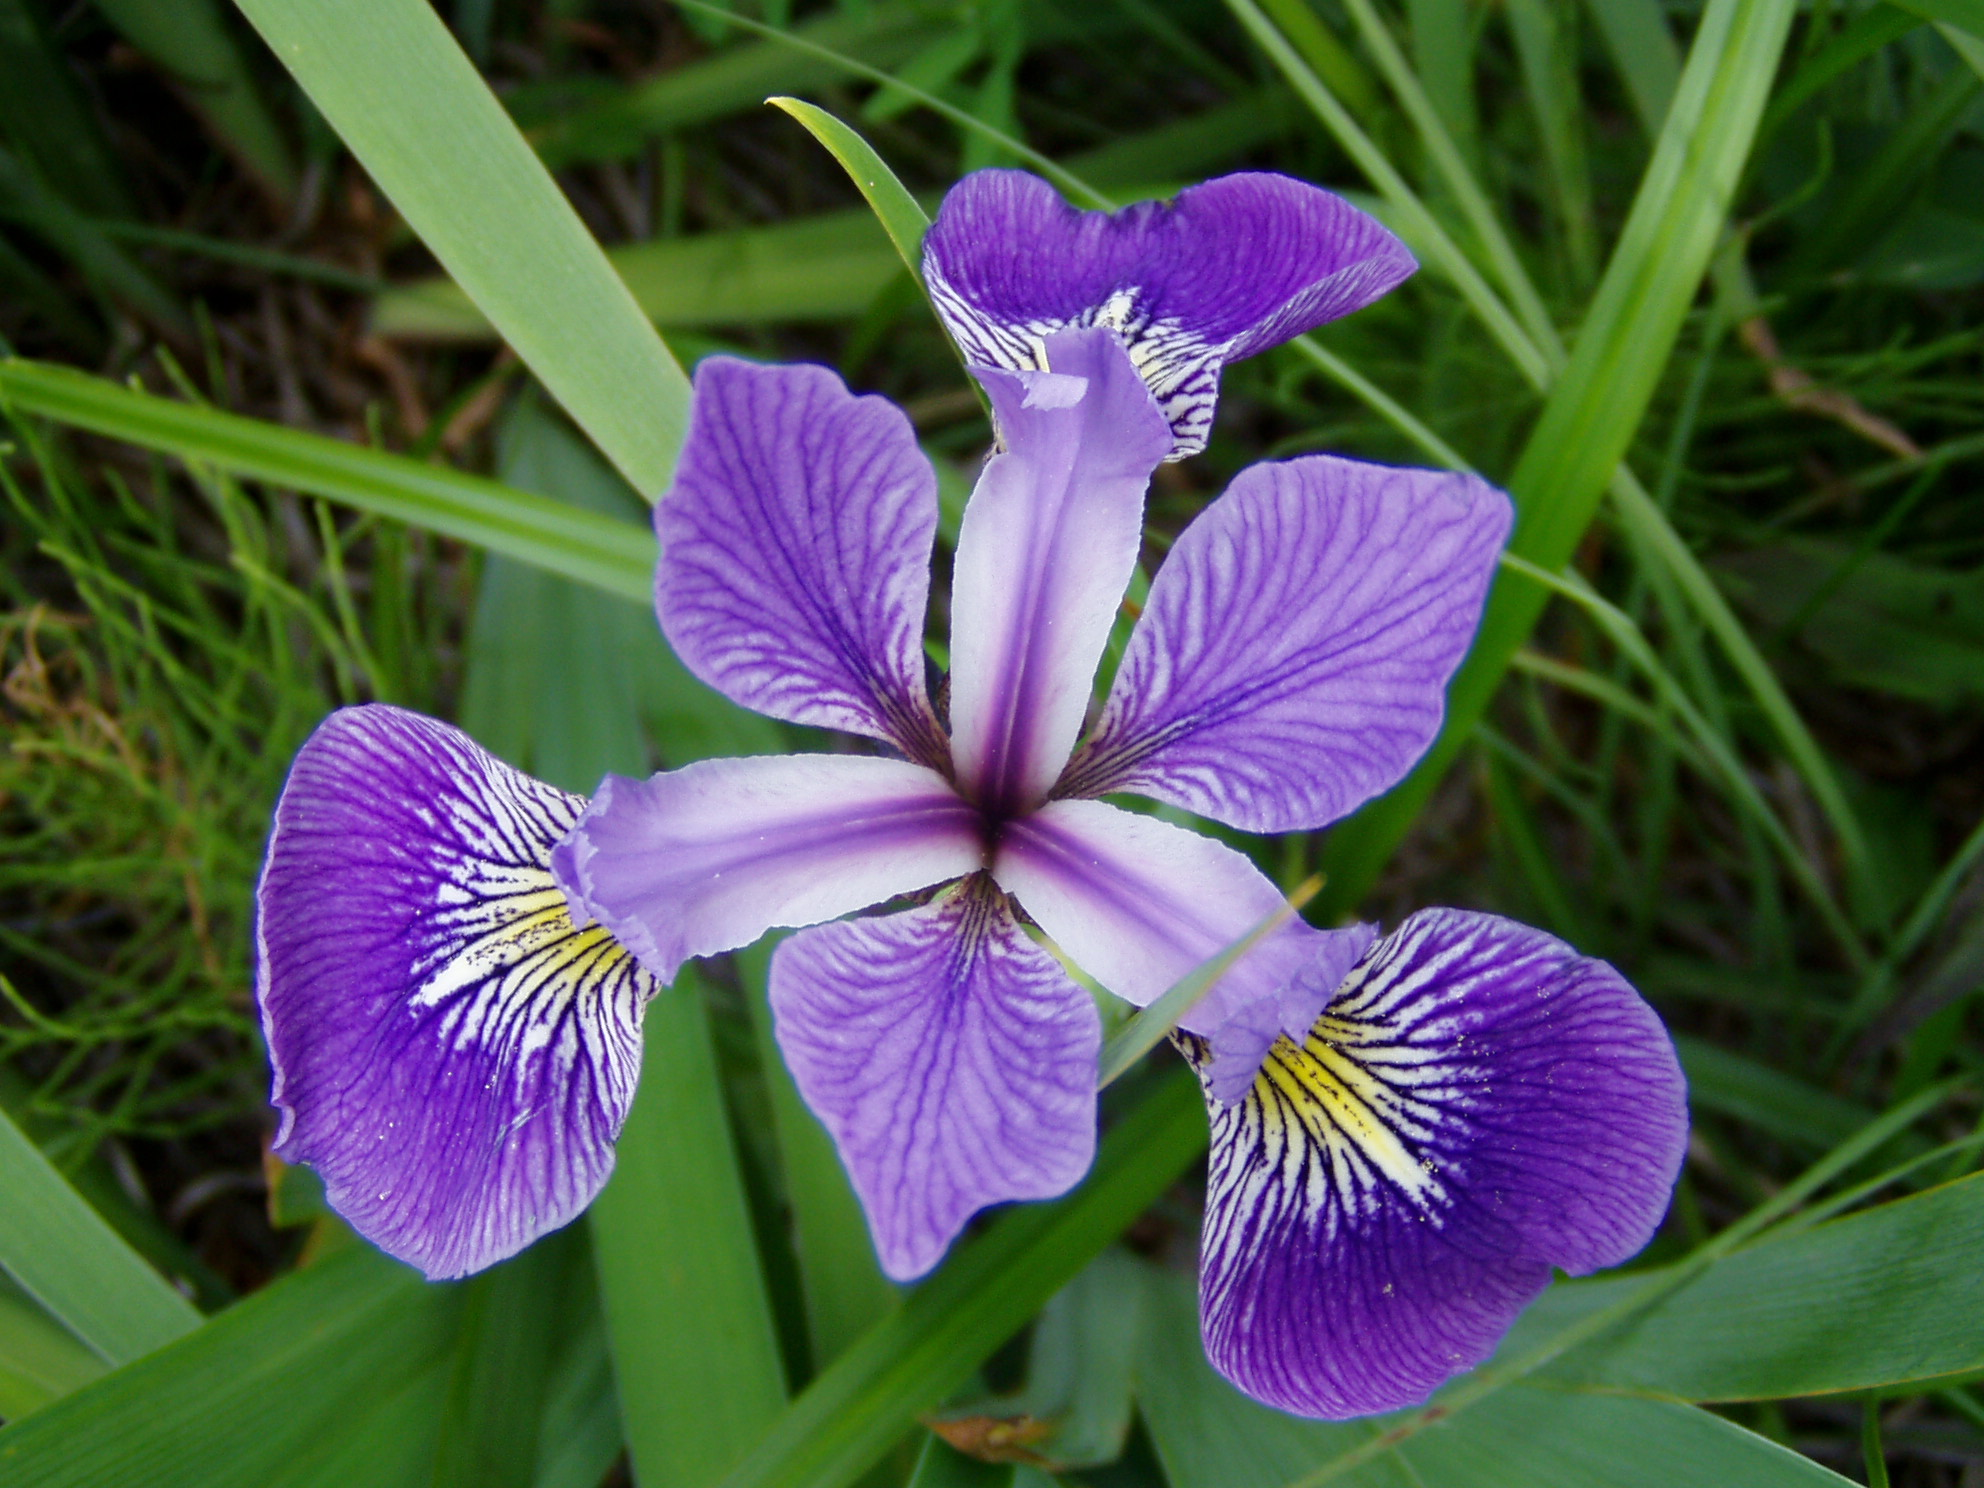
\includegraphics[width=\textwidth]{gfx/iris/Iris_versicolor_3.jpg}
			\column{0.8\textwidth}
				\begin{itemize}
					% Progettazione di un algoritmo KNN quantistico per la classificazione multiclasse
					% Implementazione sulla famiglia di processori IBM QX
					% Figura dell'IBM QX
					\item Generalizzazione di un algoritmo KNN quantistico per la classificazione multiclasse
					\item Simulare l'usabilità degli algoritmi di machine learning quantistico in contesti reali
					\item Applicazione al data set Iris (3 classi, 4 caratteristiche, 150 vettori)
				\end{itemize}
		\end{columns}
	
	\end{frame}

	\begin{frame}
		\frametitle{Machine learning}
	
		Il machine learning è una branca dell'IA che dà l'abilità ai computer di apprendere dai dati

		Gli algoritmi di machine learning permettono di apprendere modelli matematici da insiemi di 
		dati per

		\begin{itemize}
			\item effettuare previsioni su dati sconosciuti
			\item individuare regolarità nascoste
			\item compiere decisioni che danno il risultato migliore
		\end{itemize}
	
	\end{frame}

	\begin{frame}
		\frametitle{Algoritmo k-nearest neighbours}
		
		\begin{columns}
			\column{0.25\textwidth}
				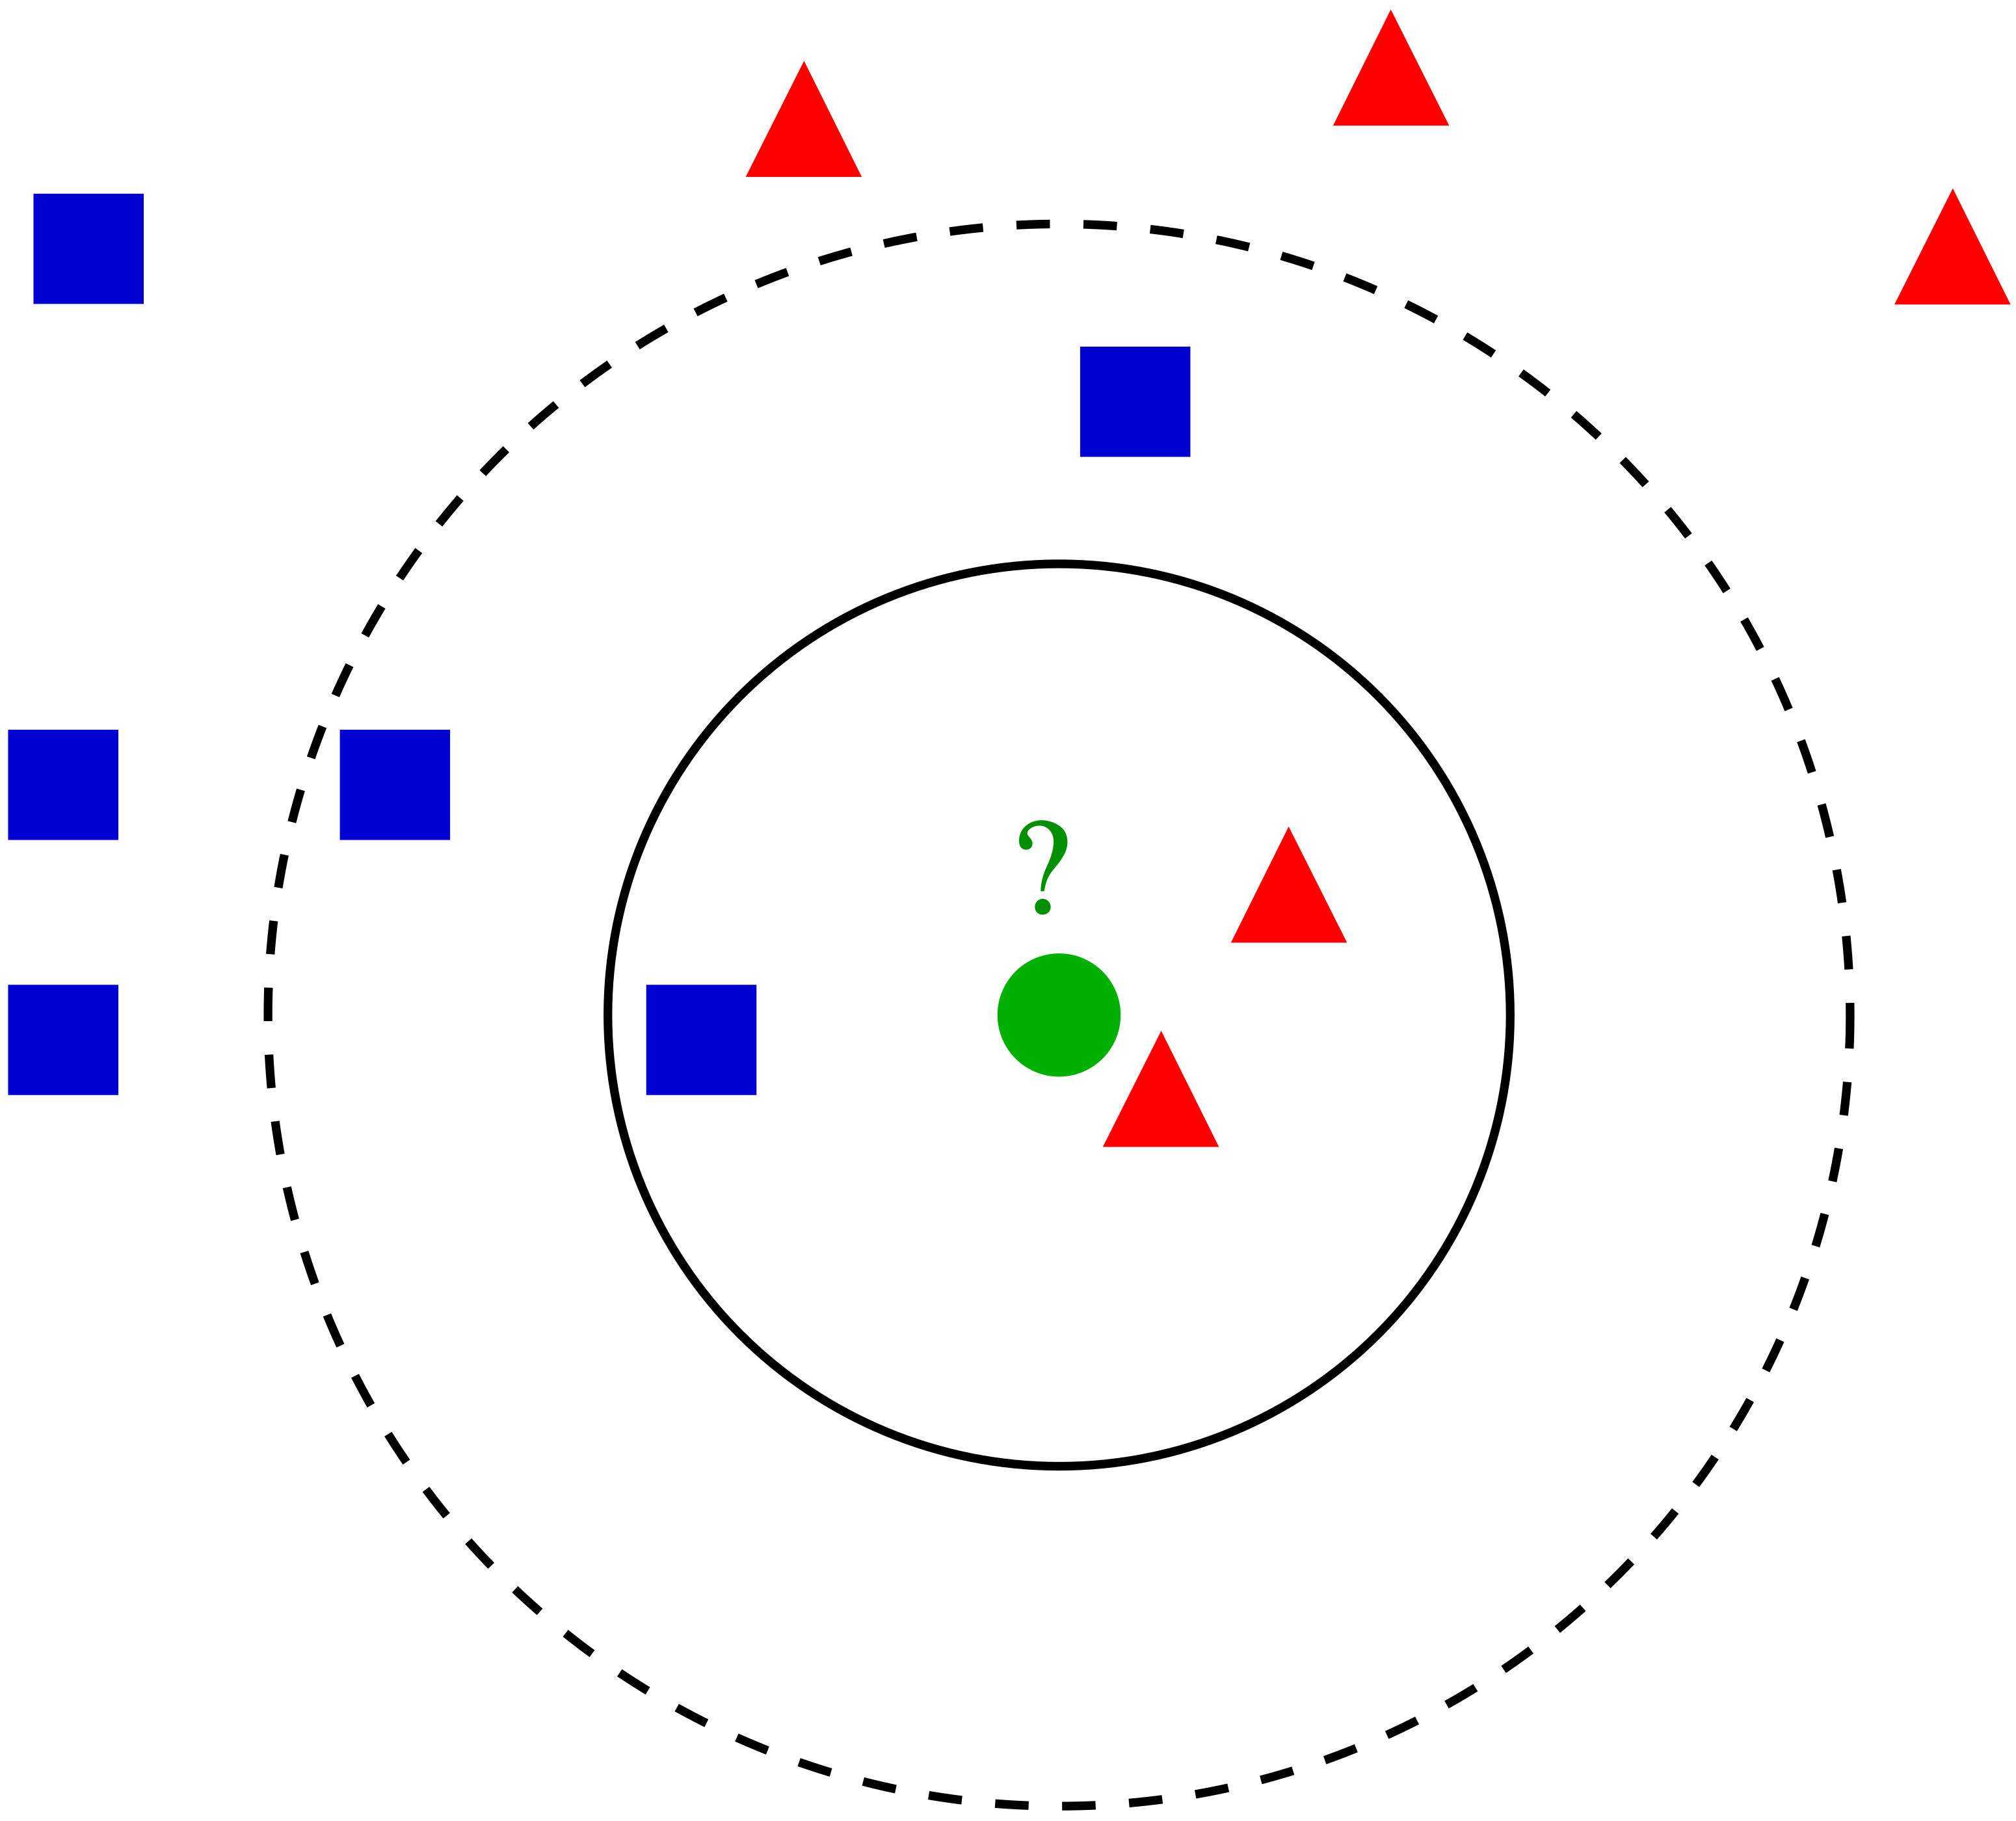
\includegraphics[width=\textwidth]{gfx/KnnClassification}
			\column{0.75\textwidth}
			\begin{itemize}
				\item $k$ è un numero naturale
				\item Dato un dataset $D = v_0, \ldots, v_n$ \\ $v_i\in\{ \text{setosa}, \text{versicolor}, \text{virginica} \}$
				\item Dato un nuovo vettore $x$
				\item Si considerano i $k$ vettori più vicini ad $x$ 
				\item Si classifica $x$ con un voto a maggioranza 
				\item Si assegnano pesi dipendenti dall'inverso della distanza per aumentare l'influenza di quelli più vicini
			\end{itemize}
		\end{columns}

	\end{frame}

	\begin{frame}
		\frametitle{Quantum computing}
	
		Usare strumenti di calcolo che sfruttano le proprietà quantistiche della materia

		\begin{itemize}
			\item Il qubit è la controparte quantistica del bit. Un bit può assumere un 
			singolo valore tra 0 e 1. Un qubit può esistere in una sovrapposizione dei 
			due stati $\ket{0}$ e $\ket{1}$. 
			\item Un qubit vive in uno spazio di Hilbert bidimensionale. 
			\item Un sistema di $n$ qubit è descritto da uno spazio di dimensione $2^n$ 
			\item Il quantum computing permette la parallelizzazione del lavoro e la 
			memorizzazione di grandi quantità di dati. 
		\end{itemize}
	
	\end{frame}

	\begin{frame}
		\frametitle{Quantum computing}
	
		Un computer quantistico con $n$ qubit possiede $2^n$ ampiezze di probabilità

		Queste ampiezze possono essere usate per immagazzinare quantità enormi di informazioni

		\vspace{1cm}

		\begin{tabular}{c c c}
			Numero di qubit & RAM classica richiesta \\ 
			\hline
			5 & 256 byte \\
			25 & 2 gigabyte \\
			50 & 8000 terabyte \\
			275 & numero di atomi nell'universo osservabile
		\end{tabular}
		
		
	\end{frame}

	\begin{frame}
		\frametitle{KNN quantistico}
		\begin{center}
			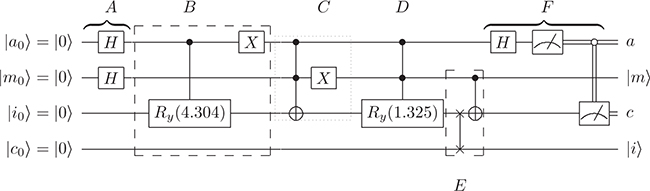
\includegraphics[width=.75\textwidth]{gfx/schuld_circuito}
		\end{center}
		
		In un articolo di ricerca, Schuld et al. propongono un algoritmo KNN quantistico 
		che permette di ridurre esponenzialmente le risorse necessarie per il riconoscimento. 

		L'algoritmo riesce a comparare due classi alla volta, usa come $k$ il numero totale di 
		vettori e usa una metrica che va come $^1/_\text{distanza}$. 

		L'implementazione viene fatta su un computer quantistico a 5 qubit. 
	
	\end{frame}

	\begin{frame}
		\frametitle{Domanda di ricerca}
		\begin{itemize}
			\item A partire dall'algoritmo KNN quantistico proposto da Schuld et al., è possible 
			implementarne una versione multiclasse?
			\item Quali sono le performance di classificazione all'aumentare del numero di qubit?
		\end{itemize}
	\end{frame}

	\section{Metodi}

	\begin{frame}
		\frametitle{IBM Q Experience}
	
		\begin{center}
			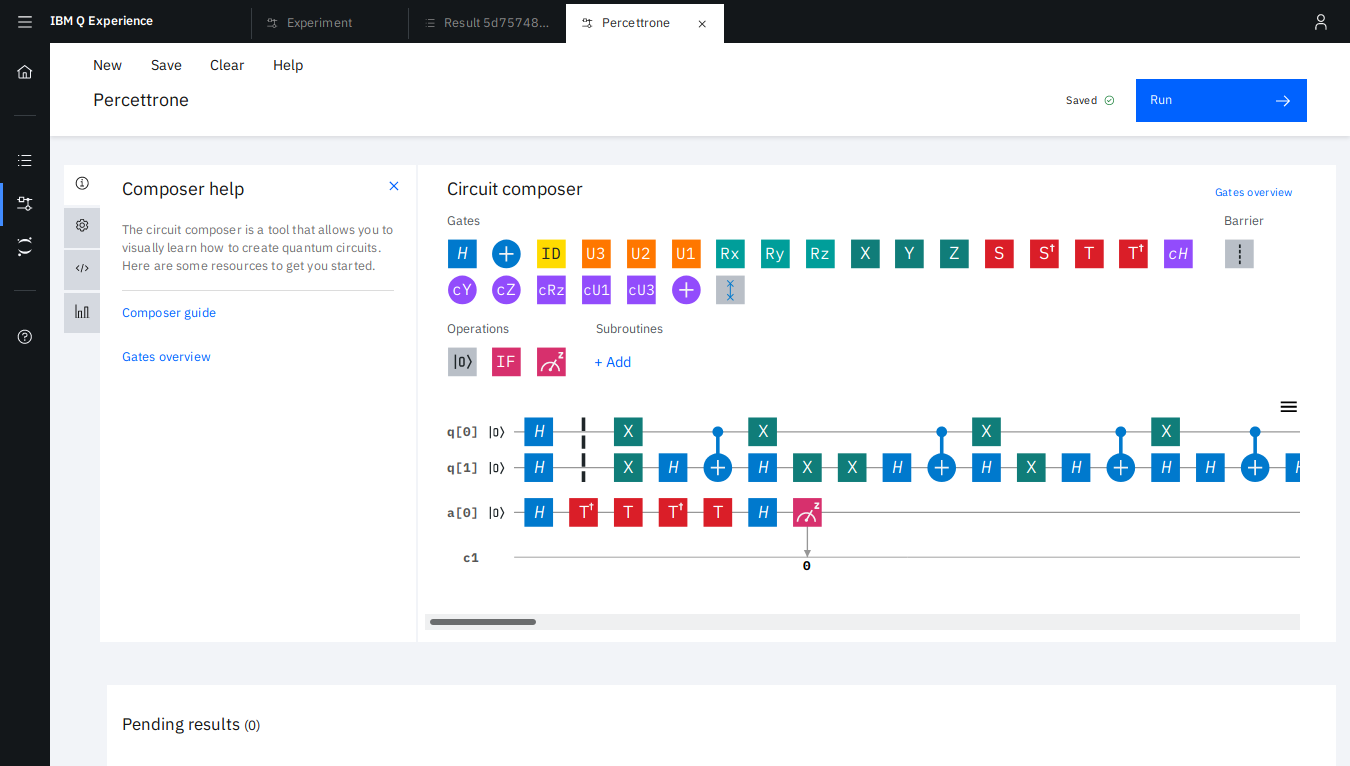
\includegraphics[width=.75\textwidth]{gfx/IBM_Q_Experience_percettrone}
		\end{center}
		\begin{itemize}
			\item Accessibile al pubblico
			\item Permette simulazioni con o senza rumore
			\item Fino a 14 qubit superconduttivi
			\item Fino a 32 qubit simulati
		\end{itemize}
		
	
	\end{frame}

	\begin{frame}
		\frametitle{Qiskit}
	
		\begin{center}
			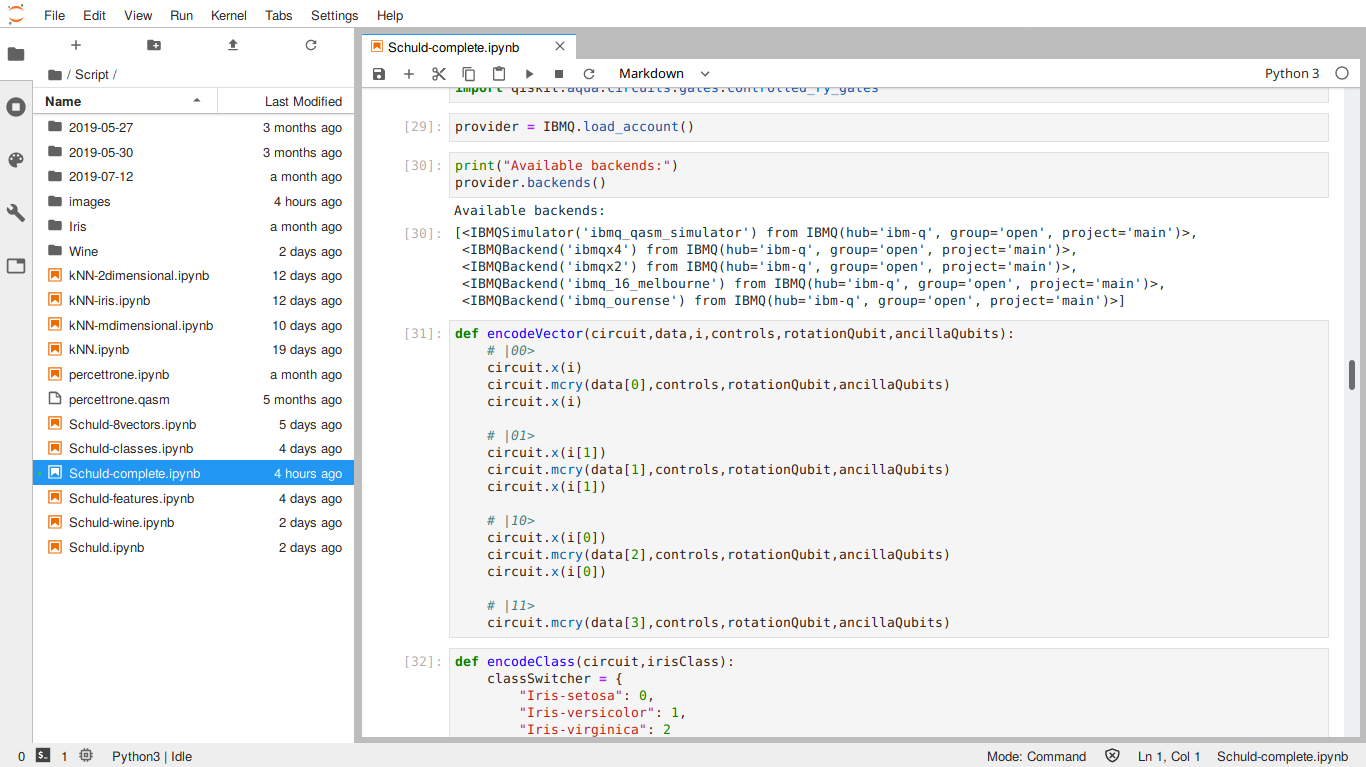
\includegraphics[width=.75\textwidth]{gfx/JupyterLab}
		\end{center}

		Piccoli circuiti quantistici possono essere simulati su computer convenzionali

		Qiskit permette di 
		\begin{itemize}
			\item ideare circuiti quantistici
			\item simularne l'esecuzione sul proprio pc
			\item interfacciarsi con l'IBM QX
			\item mandare ordini di esecuzione a veri computer quantistici
		\end{itemize}
	
	\end{frame}

	\section{Quantum machine learning}

	\begin{frame}
		\frametitle{Codificare i dati nelle ampiezze}
		
		\begin{columns}
			\column{0.4\textwidth}
				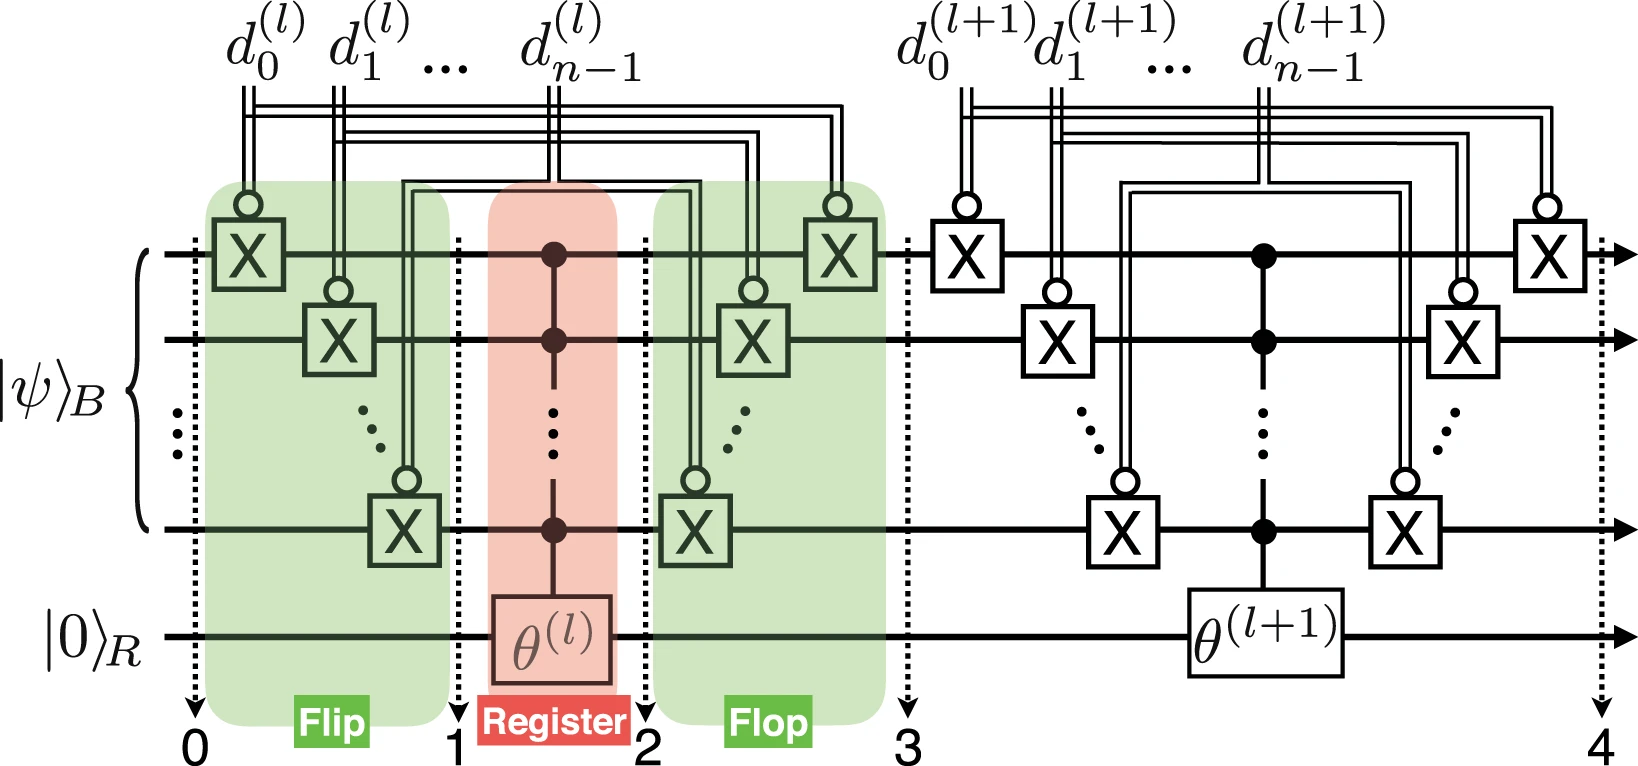
\includegraphics[width=\textwidth]{gfx/qram.png}
			\column{0.6\textwidth}
				Si è costruita una QRAM (Quantum RAM) attraverso 
				l'algoritmo di costruzione di Petruccione et al. per 
				codificare vettori classici nei vari stati quantistici 
				a disposizione
				\begin{equation*}
					\text{QRAM} \ket{0} = \ket{\psi}
				\end{equation*}
		\end{columns}
		
	\end{frame}

	\begin{frame}
		\frametitle{QKNN}
	
		Stato quantistico iniziale

		\begin{equation*}
			\ket{\psi_0} = \frac{1}{\sqrt{2M}} \sum_{m=1}^M 
			(\ket{0}\ket{\psi_x}+\ket{1}\ket{\psi_{t^m}})\ket{c^m}\ket{m}
		\end{equation*}

		Calcolo della distanza con interferenza quantistica

		\begin{equation*}
			\ket{\psi_1} = \frac{1}{2\sqrt{M}}\sum_{m=1}^M 
			(\ket{0}(\ket{\psi_x}+\ket{\psi_{t^m}})+\ket{1}(\ket{\psi_x}-\ket{\psi_{t^m}}))\ket{c^m}\ket{m}
		\end{equation*}
	
		Misura condizionale

		\begin{equation*}
			\ket{\psi_2} = \frac{1}{2\sqrt{M}} \sum_{m=1}^M \sum_{i=1}^N
			(x_i+t_i^m)\ket{0}\ket{i}\ket{c^m}\ket{m}
		\end{equation*}

		

	\end{frame}

	\begin{frame}
		\frametitle{QKNN}
	
		Probabilità di misurare una data classe

		\begin{equation*}
			P(\ket{c^m} = \ket{s}) = \sum_{m|c^m=s} 
			1 - \frac{1}{4M} |x-t^m|^2
		\end{equation*}

		Classificazione

		\begin{equation*}
			c = \begin{cases}
			0 \quad se P(\ket{c^0}) maggiore \\
			1 \quad se P(\ket{c^1}) maggiore \\
			etc\ldots
		\end{cases}
		\end{equation*}
	
	\end{frame}

	\section{Risultati}

	\begin{frame}
		\frametitle{Data set Iris}
	
		L'insieme dati usato per far girare l'algoritmo 
		è stato il ben noto Iris Data Set

		Si è prima standardizzato e normalizzato i vettori 
		di training e poi si è proceduto alla classificazione
		
		\begin{figure}[]
			\centering
			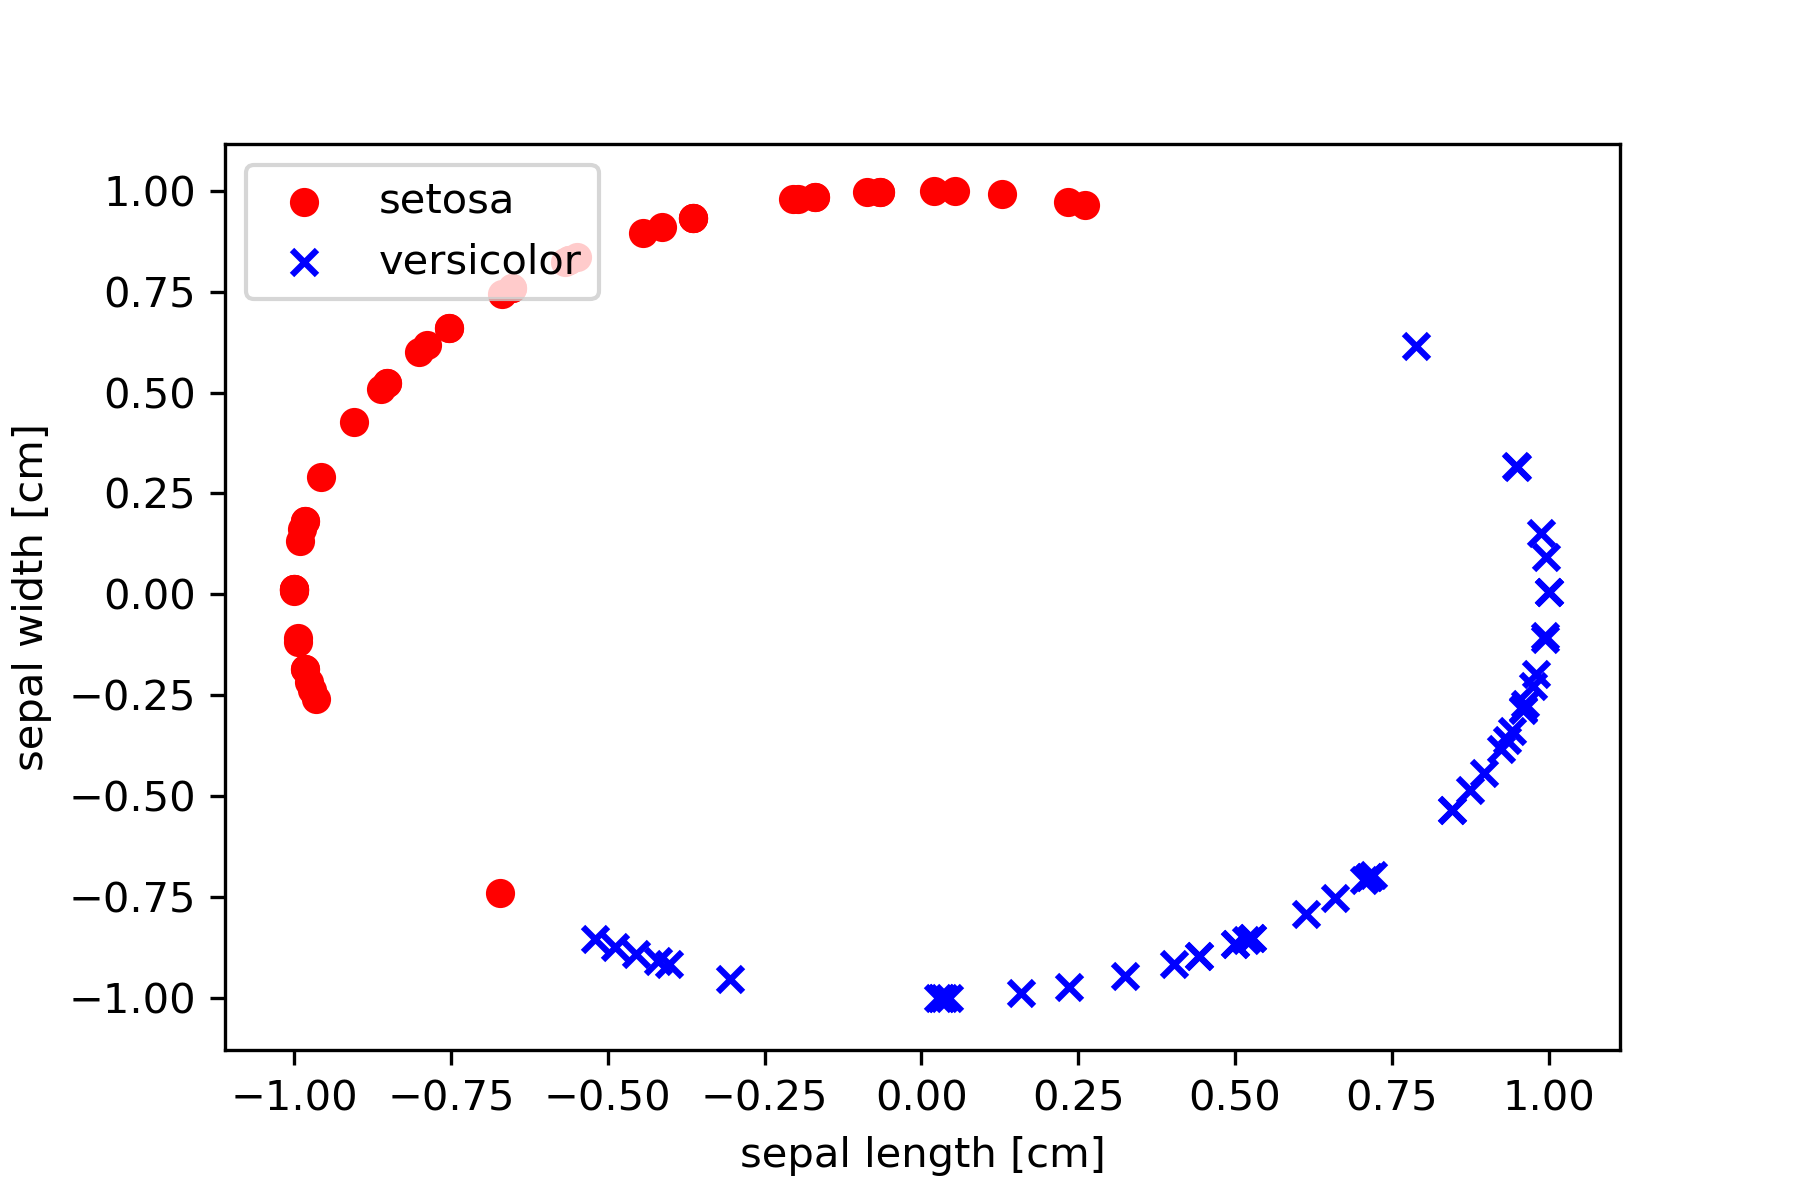
\includegraphics[width=.75\textwidth]{gfx/iris/iris2normalized}
			\caption{}
			\label{fig:iris_normalizzato}
		\end{figure}

	\end{frame}

	\begin{frame}
		\frametitle{Simulazioni}
		\begin{figure}[]
			\centering
			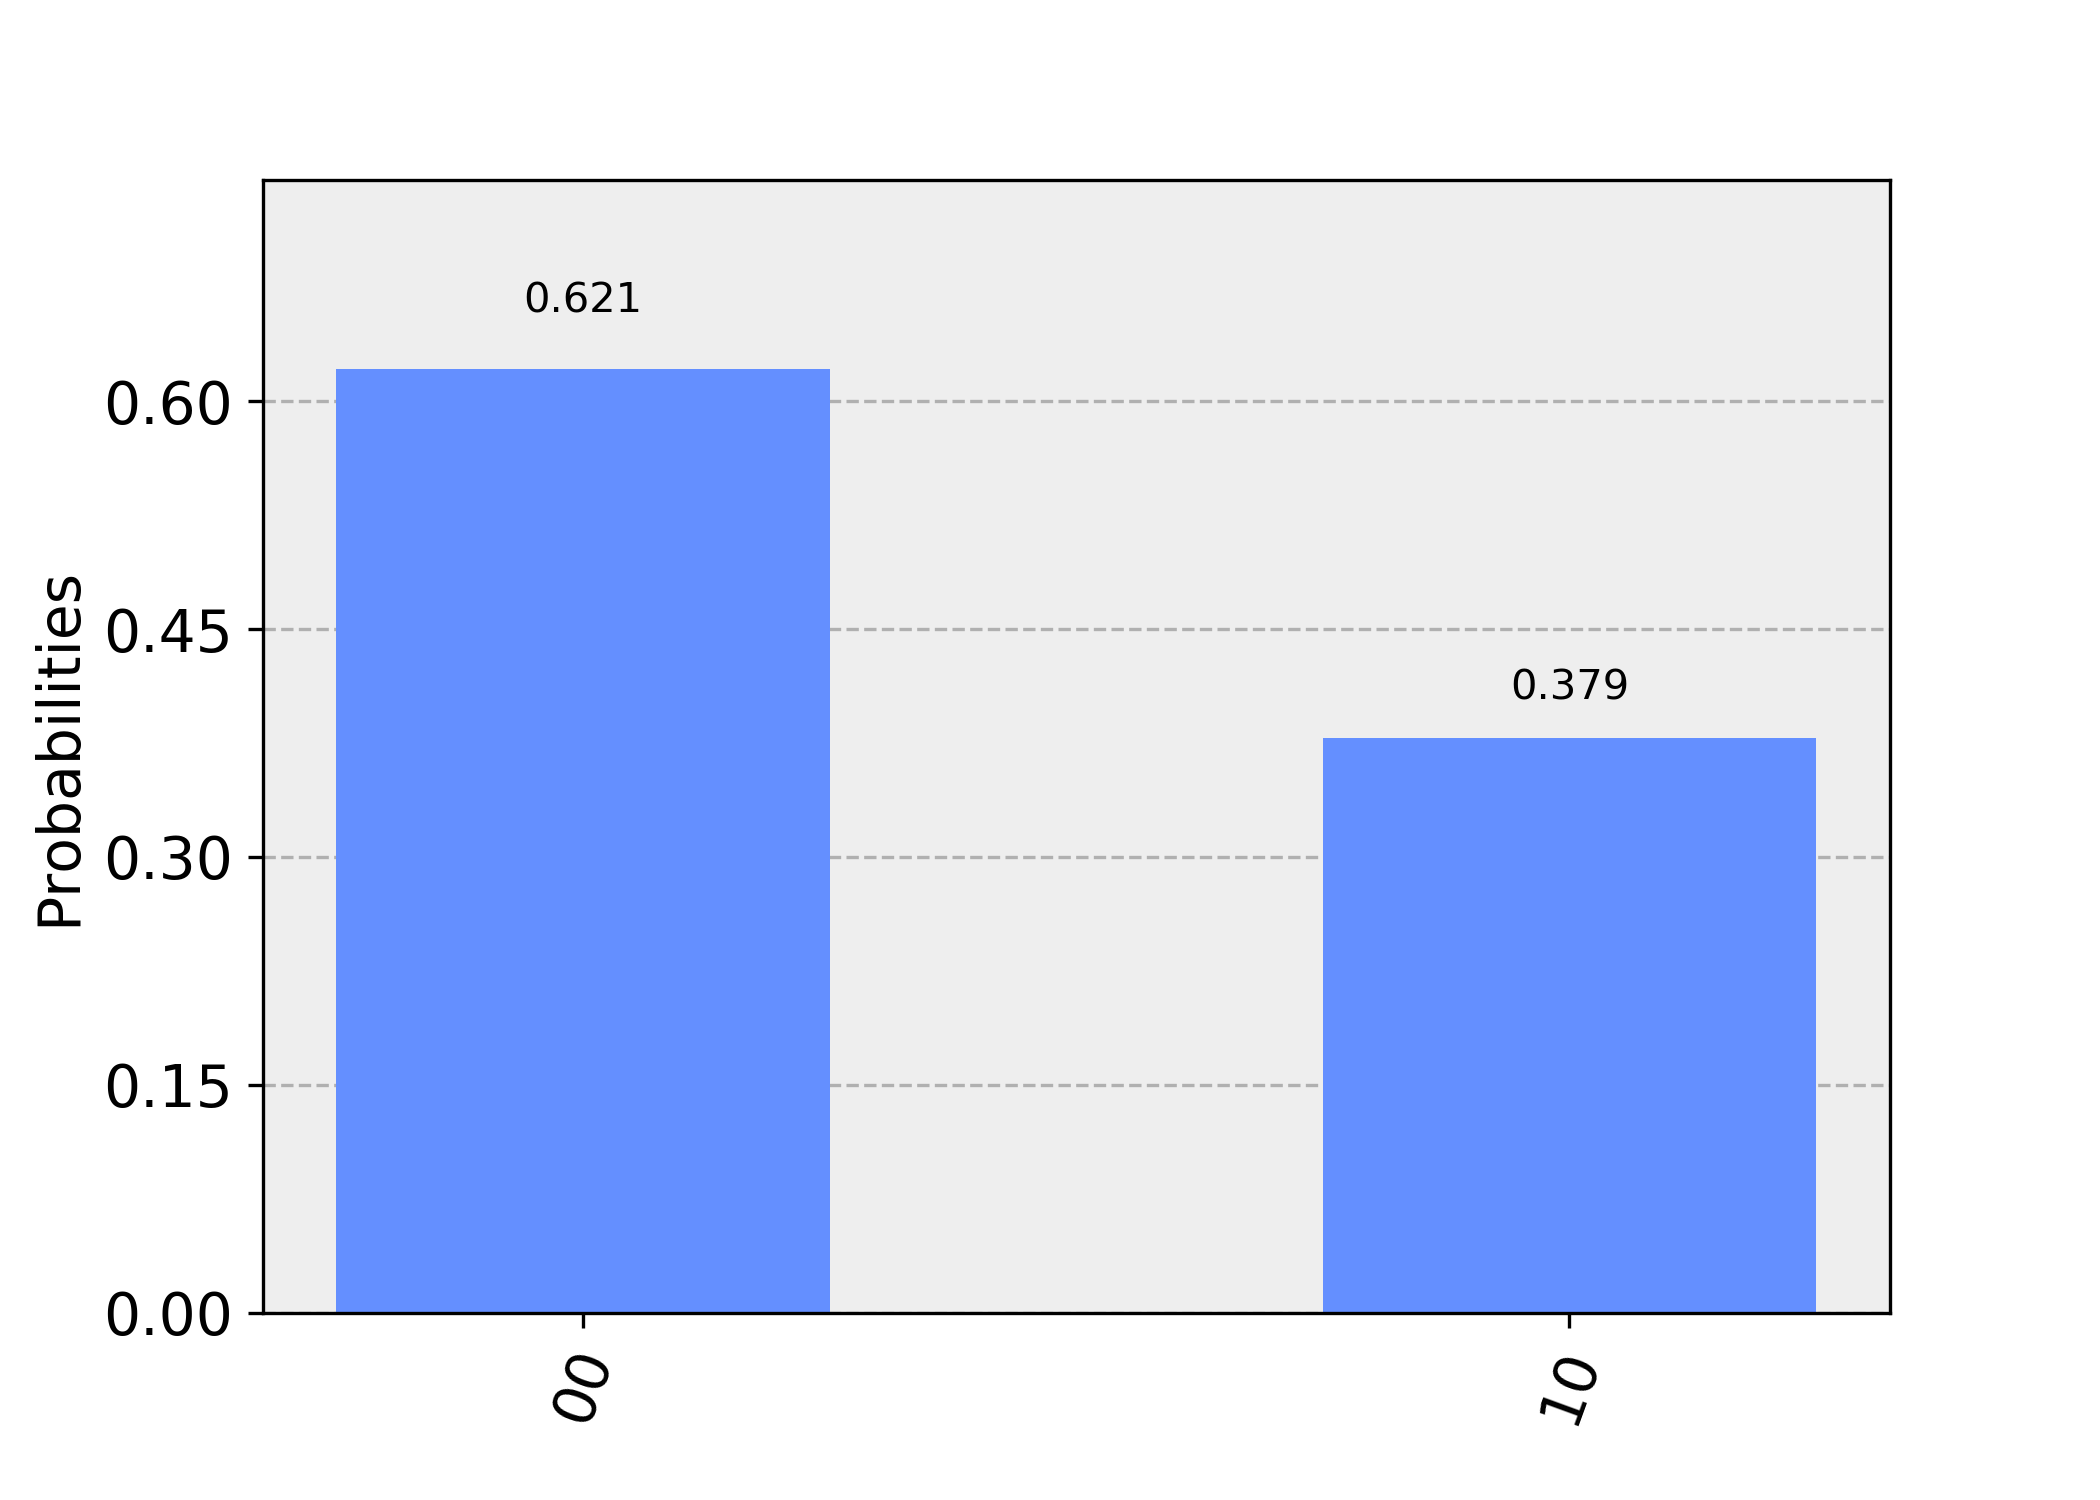
\includegraphics[width=.8\textwidth]{gfx/iris/histogram}
			\caption{Misura della classe setosa}
			\label{fig:setosa_simulazione}
		\end{figure}
	
	\end{frame}

	\begin{frame}
		\frametitle{Esecuzioni reali}
		\begin{figure}[]
			\centering
			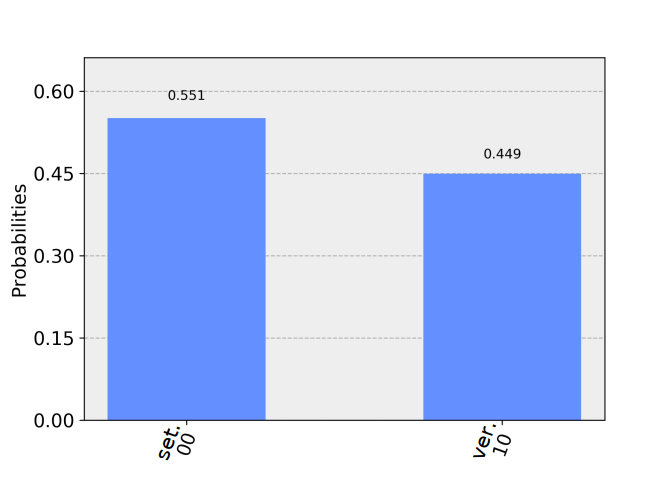
\includegraphics[width=.8\textwidth]{gfx/misura_setosa_sperimentale}
			\caption{Misura della classe setosa}
			\label{fig:setosa_sperimentale}
		\end{figure}
	\end{frame}

	\begin{frame}
		\frametitle{Classificazione multiclasse}
	
		\begin{figure}[]
			\centering
			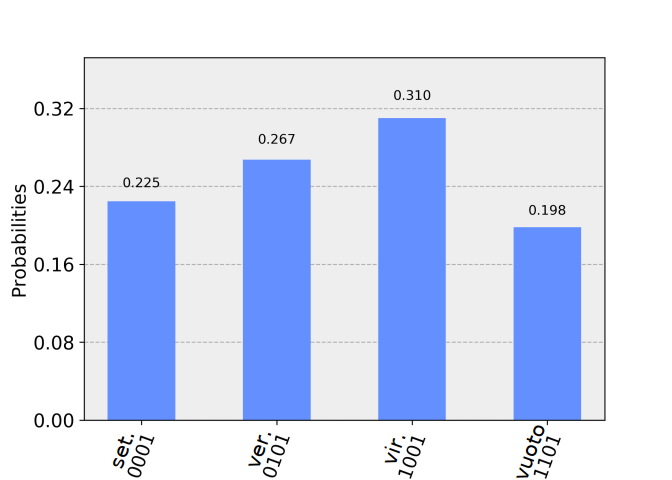
\includegraphics[width=.8\textwidth]{gfx/multiclass_virginica}
			\caption{Misura multiclasse virginica}
			\label{fig:multiclasse}
		\end{figure}
	
	\end{frame}

\begin{frame}
	\frametitle{Conclusione}

	L'implementazione rispecchia i risultati aspettati di classificazione e permette 
	di ridurre esponenzialmente le risorse necessarie in termini di memoria usata e 
	di numero di elaborazioni. 

	L'algoritmo KNN non è l'unico che può beneficiare di un'approccio quantistico e 
	si aspettano ancora molte evoluzioni nel campo del quantum machine learning. 

\end{frame}

\begin{frame}[focus]
	Domande?
\end{frame}

\end{document}